\subsection{Серверная часть}
\label{subsections:ServerImpl}

Данный подраздел содержит описание реализации серверной части приложения.
В рамках прототипа было принято решение разработать скрипт,
который, подобно конвейеру, обрабатывает исходную информационную модель
для производства пакета, содержащего все необходимые данные
(трехмерное представление здания, пригодное для производительного рендеринга;
графические материалы; извлеченная атрибутивная информация),
который может загружать используемый фреймворк визуализации.

\paragraph{Конвертация информационной модели в FBX-формат}

На первой стадии обработки производится преобразование формата модели.
Как было сказано в разделе~\ref{subsections:DomainModel},
исходный RVT-формат является проприетарной закрытой разработкой
компании Autodesk Inc., хранящей данные в бинарном формате,
что сильно затрудняет разработку парсеров для этого формата.
Помимо этого, Autodesk использует свой формат графических материалов,
которые также плохо-поддерживаются современными графическими фреймворками.

Наиболее эффективными инструментами по работе с форматами
ком\-па\-нии Auto\-desk Inc. являются её же разработки,
поэтому для выполнения преобразования был выбран редактор 3ds~Max.
3ds~Max обладает всей требуемой функциональностью, но, к сожалению,
его программный интерфейс (API) не обладает полным покрытием этой функциональности,
поэтому этот этап не удалось полностью автоматизировать при разработке прототипа.

Использование 3ds~Max для конвертации предполагает следующие шаги:

\begin{enumerate}
    \item {
        Загрузка исходной информационной модели.

        Для загрузки используется инструмент File Link Manager
        (рисунок~\ref{figure:3DCMax-FileLinkManager}),
        позволяющий загружать в 3ds~Max файлы форматов DWG, DXF, FBX и RVT.
        \begin{figure}[ht]
            \centering
            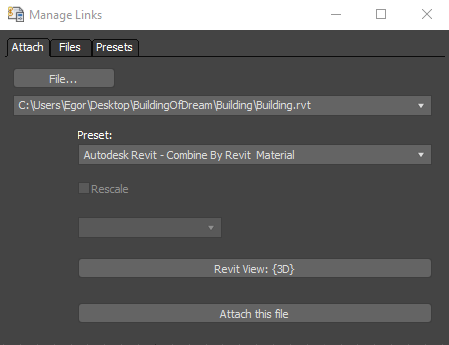
\includegraphics[width=0.5\textwidth, frame]{images/3DSMax-FLM.png}
            \caption{File Link Manager}
            \label{figure:3DCMax-FileLinkManager}
        \end{figure}
        Для загрузки необходимо выбрать загружаемый файл (Attach/File...),
        а затем выбрать одну из предустановленных опций загрузки (Preset).
        Всего на данный момент существует 5 опций,
        но в рамках прототипа нас интересуют только 2:

        \begin{itemize}
            \item {
                Autodesk Revit - Do Not Combine Entities

                При импорте с этой опцией отдельные элементы информационной модели
                будут иметь отдельные полигональные сетки, что в дальнейшем
                позволит полностью сохранить всю атрибутивную информацию.
                Недостатком этой опции является низкая финальная производительность
                и большее использование памяти для хранения такой модели
                на диске и в оперативной памяти.
            }
            \item {
                Autodesk Revit - Combine By Revit Category

                При импорте с данной опцией элементы модели, относящиеся к одной категории,
                будут объединены в одну полигональную сетку, что можно считать
                статическим батчингом модели (описано ранее
                в разделе~\ref{subsections:Optimization}).
                Такой вариант был выбран предпочтительным,
                хотя при нём неизбежно утрачивается
                значительная часть атрибутивной информации.
            }
        \end{itemize}

        После этого необходимо завершить загрузку:
        Attach/Attach this file + Files/Bind...
    }
    \item {
        Конвертация графических материалов.
        
        Для конвертации графических материалов сцены
        был использован инструмент Scene Converter (рисунок~\ref{figure:3DCMax-SceneConverter}).
        \begin{figure}[ht]
            \centering
            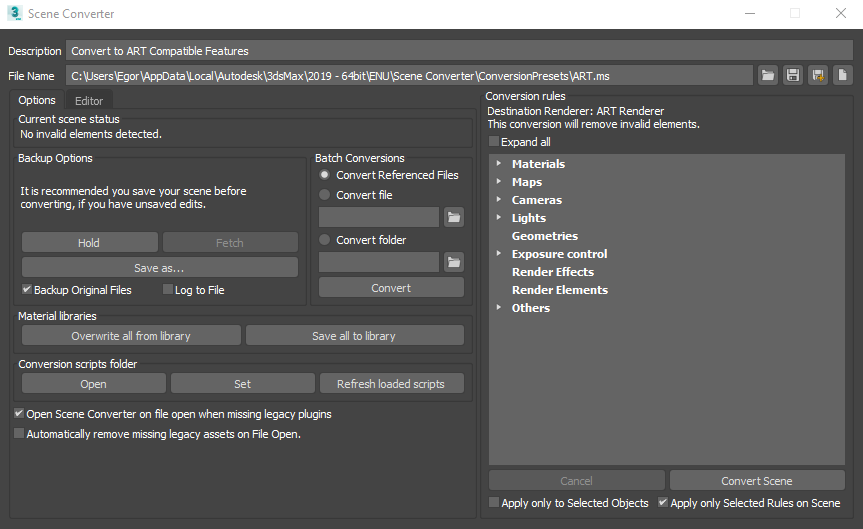
\includegraphics[width=0.8\textwidth, frame]{images/3DSMax-SC.png}
            \caption{Scene Converter}
            \label{figure:3DCMax-SceneConverter}
        \end{figure}
        Scene Converter позволяет конвертировать различные элементы сцены,
        применяя определенные правила.
        В данном случае нас интересует правило
        ``Autodesk Material to Physical Material'',
        преобразующее проприетарные графические материалы Autodesk,
        в широко используемые графические материалы,
        основанные на физических свойствах поверхности.
    }
    \item {
        Сохранение FBX модели.

        В завершение необходимо экспортировать полученную модель в FBX формате
        (рисунок~\ref{figure:3DCMax-Export}).
        \begin{figure}[ht]
            \centering
            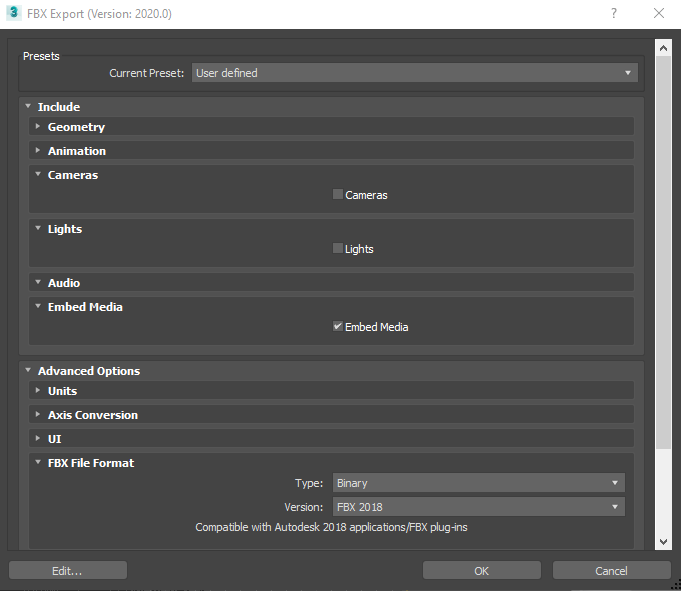
\includegraphics[width=0.7\textwidth, frame]{images/3DSMax-Export.png}
            \caption{FBX Export}
            \label{figure:3DCMax-Export}
        \end{figure}
        При сохранении необходимо исключить все анимации, камеры
        и источники света, если они присутствуют в оригинальной информационной модели,
        но сохранить встроенные медиа-данные.
    }
\end{enumerate}

\paragraph{Загрузка модели в промежуточный проект}

Приложения, разработанные на основе фреймворка Unity не имею встроенной возможности
к загрузке произвольных трехмерных моделей непосредственно с дискового накопителя.
Модели в Unity могут загружаться одним из следующих способов:

\begin{itemize}
    \item {
        Модель должна быть непосредственно загружена в проект
        разрабатываемого приложения до его компиляции.
        После этого она может загружаться в запущенном приложении
        за счет внутреннего механизма сериализации данных.
        Данный подход очевидно является неприменимым в нашем случае,
        так как он приведет к встраиванию информационной модели в приложение. 
    }
    \item {
        Загрузка модели может осуществляться за счет
        специализированного отдельно разработанного модуля,
        включенного в клиентскую часть прототипа.
        Такое решение будет слишком трудоемко для разработки в рамках прототипа. 
    }
    \item {
        Загрузка моделей может производиться с помощью встроенной в фреймворк
        системы динамической загрузки стороннего контента.
        Загружаемый контент должен предварительно упаковывать
        в специальные файлы, создание которых возможно только
        с помощью редактора Unity.
    }
\end{itemize}

Таким образом, вторым этапом обработки модели является подготовка модели к упаковке
через ее добавление в промежуточный проект редактора Unity.
К счастью, программный интерфейс редактора Unity полностью покрывает
все наши нужды, тем самым весь дальнейший процесс поддается полной автоматизации.

Для автоматического импортирования моделей в промежуточный проект
необходимо создать скрипт, который можно запускать из командной строки
без участия пользователя.\cite{DocUnity}
Общий алгоритм импорта моделей показан на рисунке~\ref{figure:SImportModels}.

\begin{figure}[ht]
    \centering
    \includegraphics[width=0.6\textwidth]{example-image}
    \caption{Импорт моделей.}
    \label{figure:SImportModels}
    \comment{ModelImport.ImportAllAssets}
\end{figure}

\intextcomment{
    Описание UML-схемы...
}

На стадии импорта моделей можно также проводить извлечение
сохранившейся в модели атрибутивной информации.
Для этого нам потребуется создать специальный обработчик моделей
(рисунок~\ref{figure:CPostprocessor}). 

\begin{figure}[ht]
    \centering
    \includegraphics[width=0.6\textwidth]{example-image}
    \caption{Постобработчик моделей.}
    \label{figure:CPostprocessor}
    \comment{AssetPostprocessor +
    ModelPreprocessor(переименовать в ModelPostprocessor) +
    ModelData + MonoBehaviour? + Dictionary}
\end{figure}

\intextcomment{
    Описание UML-схемы...
} Сам процесс извлечения атрибутивной информации показан
на рисунке~\ref{figure:SPostprocessor}.

\begin{figure}[ht]
    \centering
    \includegraphics[width=0.6\textwidth]{example-image}
    \caption{Извлечение атрибутивной информации модели.}
    \label{figure:SPostprocessor}
    \comment{ModelPreprocessor.OnPostprocessGameObjectWithUserProperties}
\end{figure}

\intextcomment{
    Описание UML-схемы...
}

\paragraph{Упаковка моделей}

Финальным шагом обработки информационных моделей является упаковка.
Для этого был выбран механизм фреймворка Unity называющийся AssetBundle.
AssetBundle это архив, содержащий не скриптовые ресурсы,
например модели или текстуры, который можно динамически загружать
или выгружать в момент выполнения приложения.
Пакеты могут обладать взаимными зависимостями, например графический материал,
упакованный в один AssetBundle может использовать текстуру,
упакованную в другой AssetBundle (рисунок~\ref{figure:AssetBundleDependency}),
что может сильно уменьшить расход памяти, если таких пакетов
с графическими материалами станет несколько.%
\cite{DocUnity,UnityAssetsResourcesBundles}

\begin{figure}[ht]
    \centering
    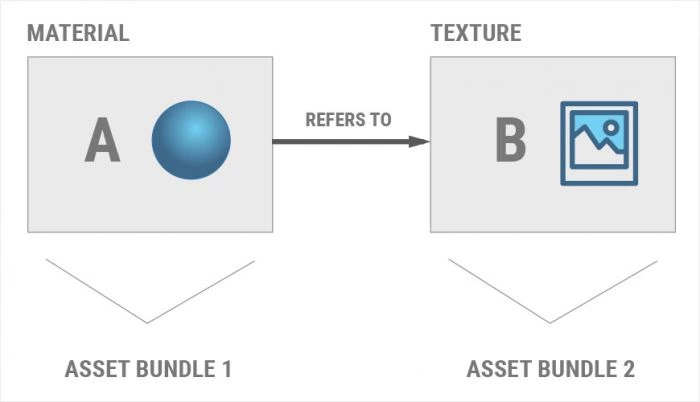
\includegraphics[width=0.8\textwidth]{images/AssetBundleDependency.png}
    \caption{Взаимозависимости ресурсных пакетов.%
    \cite{UnityAssetsResourcesBundles}}
    \label{figure:AssetBundleDependency}
\end{figure}

Помимо этого AssetBundle обладает встроенными механизмами сжатия,
а также механизмами версионности и кеширования,
что позволит эффективнее справляться с модификациями информационной модели.%
\cite{DocUnity,UnityAssetsResourcesBundles}
Создание ресурсных пакетов тоже может быть полностью автоматическим,
что показано на рисунке~\ref{figure:SExportBundles}.

\begin{figure}[ht]
    \centering
    \includegraphics[width=0.6\textwidth]{example-image}
    \caption{Экспорт пакетов}
    \label{figure:SExportBundles}
    \comment{ModelImport.ExportAssetBundles}
\end{figure}

\intextcomment{
    Описание UML-схемы...
}

\comment{
    TODO:

    Запилить UML!

    скрипты смотреть тут
        C:\Users\Egor\Rubius\model-import-test\Assets\Scripts\ModelImport\Editor
}
